\chapter{极限}

\begin{figure}[ht]
  \centering
  \includegraphics[width=1\textwidth]{asset/茶桁的 AI 秘籍_Math_7.png}
\end{figure}

\newpage

今天的课程还是微积分系列课程中的一节. 上一节课我们详细介绍了一下函数, 给大家解释了函数的本质. 这节课我们要来讲一下微积分里的另外一个概念: 极限. 

在这节课中, 我们会看到一些公式, 我还会带着大家推导一些东西. 

\section{极限}

首先说一下极限这个概念. 

极限这个词我们已经听过很多次了, 就是什么趋近什么的极限, 在这个点的附近极限等于多少多少. 大家都听过很多诸如此类的这种描述. 

那我们怎么样从数学的角度去严谨严密的描述极限是怎么一回事呢?什么样才叫无限逼近某一个量?以及这个量可以到达吗?也就是说, 极限我可以取到吗?还是说我永远只能逼近他, 却永远达不到. 这听着就感觉有点伤感, 就像一个男生追一个女生永远追不到.

首先来看一下极限正式的定义: 

\begin{newquotation}
  设函数$f(x)$在点$x_0$附近有定义, 如果存在常数$a$, 对于任意给定的正数$\varepsilon$, 都存在正数$\delta$, 使得对于任意$x$满足$0<|x-x_0| < \delta$, 均有$|f(x)-a| < \varepsilon$, 则称常数$a$为$f(x)$在$x$趋近于$x_0$时的极限, 记作: 
  \begin{align*}
    \lim_{x-x_0}f(x) = a
  \end{align*}
\end{newquotation}

以上定义是一段极限的标准定义, 对于极限除了标准定义之外还有「左极限」和「右极限」这两个概念, 分别为 左极限: $\lim_{x-x_0^{-0}}$, 右极限:$\lim_{x-x_0^{+0}}$. 不过对比下来发现, 其实我们平时所求的极限, 本质上都是先求了左右极限, 然后二者相等, 才得到了我们的函数极限. 也就是说, 如果左右极限不相等, 那么函数在这个点上极限不存在. 而且平时我们也很少先求左右极限再比较得到极限. 

还是来继续讲解极限. 我们先用一段非常数学化的语言去描述一下极限正式定义: 设有一个函数$f(x)$在点$x_0$附近有定义, 「有定义」就是$f(x)$在$x_0$附近都可以映射. 如果存在一个常数$a$满足下面的条件, 任意给一个正数$\varepsilon$, 不管这个正数多大还是多小, 只要是任意的, 都存在另外一个数$\delta$, 并且也是一个正数, 使得$|f(x)-a|<\varepsilon$. 就是$f(x)$和$a$相减的绝对值小于$\varepsilon$小于你任意给的这个数$\varepsilon$这个结论在$|x-x_0|$属于$(0, \delta)$ 这个区间之内的时候恒成立. 如果这样的话, 我们就把常数$a$称为$f(x)$在趋近于$x_0$时的极限. 

不要发懵, 我们来详细解释一下. 

首先来看$x_0$附近的定义, 所谓$x_0$附近, 实际上就是指一个以$x_0$为中心的「去心邻域」. 

那什么是「去心邻域」呢?我们来拿一个数列说明一下: 

\begin{align*}
  [-5,-4,-3,-2,-1,0,1,2,3,4,5]
\end{align*}

在这一组数列中, 假设 0 就是$x_0$, 那么这整个数列就都是$x_0$的邻域. 如果关心它的半径, 这段去心邻域的半径就是 5. 因为现在给定的是一个确定的数列所以半径我们知道, 但是大部分时候我们并不知道这个$x_0$的邻域是多少, 所以可以用$\delta$来替代, 也就写成$(x_0, \delta)$, 这个$\delta$当前并不是在这个数列中的任意值, 而是一个半径值. 如果用图像表示, 可以表示为图\ref{fig:img8_1}这样: 

\begin{figure}[ht]
  \centering
  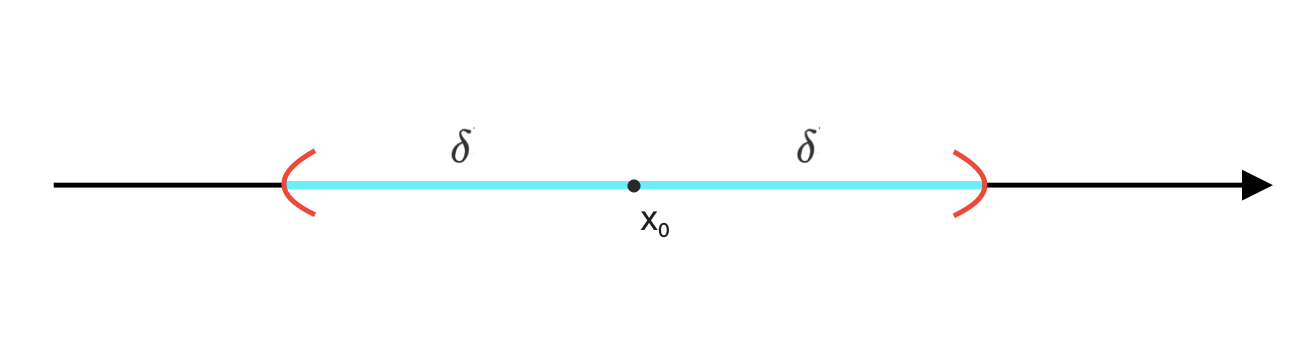
\includegraphics[width=1\textwidth]{asset/c1569200-3866-4cf7-8ec1-6cc23521eaff.png}
  \caption{$x_0$及其邻域}
  \label{fig:img8_1}
\end{figure}

那在这个图像中如果去掉$x_0$这个中心点, 就是$x_0$的去心邻域, 也就是定义里的「$x_0$ 附近」. 

之前已经说了, 在点$x_0$的附近这个函数都可以映射, 这些点就相当于$x_0$附近的这些点. 都是我们的手, 这些蜡烛的光都可以照到, 函数的规则都可以映射到. 

$\varepsilon$是任意给定的, 无论这个$\varepsilon$多么小, 小到令人发指的程度, 如果存在常数$a$, 求$|f(x)-a| < \varepsilon$都能成立. 

只需要一个条件, 就是先找到一个正数$\delta$. $|x-x_0|$ 是在$(0,\delta)$ 这个区间范围内. 这个区间范围内就是 $0<|x-x_0|<\delta$, 一个开区间\footnote{开区间, 高一知识点. 开区间用圆括号表示, 表示这个端点取不到. 如果是用方括号来表示, 就表示端点值可以取到, 那就是闭区间.}. 我们之前已经说过了, $\delta$是一个半径取值, 从理论上来说, $\delta$是不可能为负数的. 

所以只要我能找到这么一个正数$\delta$, $|x-x_0|$ 在 $(0, \delta)$ 范围之内不管$\varepsilon$有多么小都可以满足$|f(x) - a| < \varepsilon$. 那我们就可以得到这样的结论:$\lim_{x-x_0}f(x) = a$, 我们就说$f(x)$它在$x$趋近于$x_0$的时候极限为$a$, 这个常数$a$就是这个函数在这一点的极限.

在这个定义中, $x_0$和常数$a$都类似于基准点, 而$\delta$和$\varepsilon$都类似于精度. 这个定义的意思是, 给定任何一个需要达到的精度$\varepsilon$(即$|f(x)-a|$)都能找到一个$\delta$, 使得在$x_0$去心邻域这么小的范围内, $f(x)$均在$\varepsilon$精度内. 也就是说, 当不断缩小$f(x)$的范围的时候, 总能通过缩小$x$的范围, 使得$f(x)$落在给定的范围内. 

这个是比较绕的. 下面我带大家先看一下这个例子, 如果大家一时还看不太懂没有关系, 也不要慌, 先来看一个简单一点的: 

\begin{align*}
  x\in [-1, 1], \lim_{x \to 0} x = ?
\end{align*}

那这个式子里,这个函数 y 就等于 x, 我们弄一个最简单一个函数. 先告诉你这 x 的取值范围是[-1,1], 就是说, 我们手的范围就是这么大, 这个蜡烛的光只能照到这个范围. -2 照不照得到呢?照不到,那 2 照不照得到呢, 也照不到. 然后我们考虑当$x$趋向于 0 的时候($x\to0$), 这个式子的极限是多少.

首先大家可以看一下. 从直觉上面判断既然$x$可以取到 0 了, 这个 0 不就是在-1 到 1 之间吗?所以既然能取到逼近他的时候, 这极限的趋势当然就是 0 了. 

那我们接下来再看第二个: 

\begin{align*}
  x \in [-1,0) \cup (0, 1], \lim_{x \to 0} x = ?
\end{align*}

那这个式子里, 我们把 0 给去掉了. 这个$\cup$符号呢叫做并集,表示把这两个集合或者说区间给它并在一起. 并在一起之后这两个就都是我们手的范围了. 

那现在问题来了,0 现在取不到了, 不属于这个区间. 那我这个时候$x$的极限在这一点会是什么样的情况呢?

首先,我们先猜想一下它的极限值为$a=0$, 别急, 我们只是先猜想一下. 然后按照这个定义我们任意取一个$\varepsilon$, 任取一个, 随便怎么取都行. 然后我们令$\delta$等于$\frac{\varepsilon}{2}$, 这个是符合我们定义的, $\varepsilon$是任意的,$\delta$是可以自己取, 因为定义里面$\delta$只要存在一个就行了, 只要能找着. 

那你就可以自己去添加一些性质, $\delta = \frac{\varepsilon}{2}$, 这个当然也是大于 0 的, 所以我们来看一步步的, 严格按照极限的这个定义来看的话, 当$|x-x_0|$落在了大于 0,小于$\delta$这个范围之内. 

\begin{align*}
  0 < |x-x_0| < \delta
\end{align*}

我来解释一下, 为什么要让这个绝对值大于 0 呢?为什么不能等于 0 呢?等于 0 其实对应的什么样的情况, 就是$x=x_0$. 如果它们相等, 就跟我们刚才第一个式子里一样了, 都可以取到. 那你这时候来讨论极限就没什么意思了. 大家都知道 1+1=2,现在拿这个考大学生没什么意思了对吧?

所以我们把这个等于给它去掉, 让它大于 0, 小于$\delta$这个范围. 我们把$\delta$再换一下, 用$\delta = \frac{\varepsilon}{2}$这个式子再换一下, 它就变成了这么一个式子: 

\begin{align*}
  0 < |x - 0| < \frac{\varepsilon}{2} \\
\end{align*}

好,那我们再来看一下: 

\begin{align*}
  |f(x)-a| = |x - 0| < \frac{\varepsilon}{2} < \varepsilon
\end{align*}


这时候$f(x)-a$不就是$x-0$么?$f(x)$就是$x$, a 我们假设它就是 0. 所以在这里我们得到的$|x-0|$, 其实不就是上面式子$0<|x-0|<\frac{\varepsilon}{2}$中的$|x-0|$吗? 我们已经知道它是小于$\frac{\varepsilon}{2}$的, 那它肯定是小于$\varepsilon$. 所以就证明出来, 只要$|x-x_0|$在$(0, \varepsilon)$这个范围内, 这个函数$f(x)$减去它的极限$a$就小于$\varepsilon$. 就证明出来了它的极限值确实是 0. 

\begin{align*}
  \lim_{x \to 0} x = 0
\end{align*}

那我下面呢,就给大家一个完整的求值过程: 

\begin{align*}
  & x \in [-1,0) \cup (0, 1], \lim_{x \to 0} x = ? \\
  & \mbox{解:  (按照极限定义)}\\
  & \mbox{猜想其极限值为}a = 0, \mbox{取任意}\varepsilon > 0, \mbox{令} \delta = \frac{\varepsilon}{2} > 0 \\
  & \mbox{则,当} 0 < |x-x_0| < \delta, \mbox{即} 0<|x-0| < \frac{\varepsilon}{2} \mbox{时},\\
  & |f(x) - a| = |x - 0| < \frac{\varepsilon}{2} < \varepsilon \\
  & \mbox{所以} \lim_{x \to 0} x = 0
\end{align*}

看到这里, 有些小伙伴可能会比较懵. 其实这一部分如果实在理解不了, 也可以暂时先放在一边不用去管它. 我们知道极限是一个什么样的东西就可以了: \textit{它代表一种无限逼近的一个过程}. 知道这点, 就 OK 了. 至于这个理论推导, 包括证明, 其实大家不用太 care 它. 

整个证明的过程, 其实核心思想就是$\varepsilon$得是任意的,$\varepsilon$控制不了.  别人给你一个$\varepsilon$, 不管什么$\varepsilon$, 都得满足这个上面的式子. 

所以, 我们在证明过程中, 取值用了一个词「任意」.  用「任意」去表示它. 但是在$\delta$这里, 为什么我们可以令它是$\frac{\varepsilon}{2}$,其实我们在这里令它是$\frac{\varepsilon}{3}$、$\frac{\varepsilon}{4}$, 甚至其他什么式子都可以, 没有关系. 因为定义里面说了, 虽然$\varepsilon$是任意给的控制不了, 但是这个$\delta$只要能找到这么一个, 哪怕只能找到一个,它是一个正数, 使得$|x-x_0|$落在$(0,\delta)$这个范围之内就能推导出$|f(x) - a| = |x - 0| < \frac{\varepsilon}{2} < \varepsilon$. 如果能找到这样的$\delta$就可以说它的极限等于啥啥啥. 

所以我们比较能操作的部分就在于这个$\delta$的选取,这个选取可以自由发挥. 当然了,最终的目的还是在倒数第二步里, 能用关系推导出来$|f(x)-1| < \varepsilon$就可以了. 

整个过程似乎看着很随意是吧?随便弄了一个$\delta$, 然后就\textit{kua kua kua}写式子, 就证明出来相等了, 这样感觉好像不对. 

那我们就来看一个反例, 来说一下为什么上面这个极限表达的极限不是 0.1. 

\begin{align*}
  & x \in [-1,0) \cup (0, 1], \lim_{x \to 0} x = ? \\
  & \mbox{思考:  为什么 0.1 不是其极限值?}\\
  & \mbox{假设其极限值为}a = 0.1, \mbox{取} \varepsilon = 0.05, \mbox{对任意}\delta > 0, \\
  & \mbox{则当} 0< |x-x_0| < min\{\delta, \varepsilon \}, \mbox{即}|x-0| \in (0, 0.05)\mbox{时} \\
  & \mbox{有}-0.05 < x < 0, \mbox{或} 0 < x < 0.05 \mbox{时} \\
  & |f(x)-a| = |x-0.1| \in (0.05, 0.15) \Rightarrow |x-0.1| > 0.05 = \varepsilon \\
  & \mbox{所以} \lim_{x \to 0} x \ne 0.1
\end{align*}

我们先用反正法来来看一下, 先假设它就等于 0.1. 这时候取$\varepsilon = 0.05$, 对任意$\delta > 0$. 大家看到这里可能会迷糊, 刚才那个证明里面不是说$\varepsilon$是别人强塞给你的, 任意的, 别人给啥你都得接受吗? 那怎么这里$\varepsilon$可以自己取了? 刚才$\delta$不是可以自己取的吗, 怎么现在$\delta$控制不了, 得是任意的, 别人强塞给你什么你都得接受了?

这个, 涉及到命题里面的的「否命题」这么一个概念. 命题逻辑这部分知识说如果我们把一个命题取否的话, 那原来它那个文字表述里面写着任意两个字的地方全部要改成存在. 原来存在的地方都要改成任意, 这是一种相互对称的关系. 我鼓励大家自己去搜一下, 命题的否定, 否命题. 

因为我们要证明它不是一个极限, 所以这里就和刚才反着来, $\varepsilon$随便找一个, 任意的$\delta$大于 0,当我这个$|x-x_0|$处于$ 0< |x-x_0| < min\{\delta, \varepsilon \}$范围之内的时候. 

接下来这里可能又有点迷糊人,$min\{\delta, \varepsilon\}$嘛意思, 这个式子表示什么? 这个花括号里面组成了一个集合, $min$表示我取这个集合里面的最小值. 在这里就表示在这两个数里面取一个最小值的意思. 

那为什么要添加这个东西呢? 这也是一个比较困难的地方, 就是$\delta$确实是任意的, 别人强制性塞给我, 我必须得接受的. 但是我可以同样采取一个比较巧妙的一个措施. 的确这个$\delta$扔给我之后, 其实我们真正关心的是$x$和$x_0$非常接近的情况. 因为当$x$和$x_0$差很多的时候, 极限肯定也差的很多. 

就像图像上面两个点,连续函数图像,如果两个点差的特别远,那他们的函数值肯定也会差的比较远. 但是如果两个点挨的比较近,那函数值也比较接近. 

所以虽然$\delta > 0$, 但其实我们认为真正有用的部分是$\delta$非常非常小的时候. 所以在这里弄一个$min$,就控制了$\delta$再大,至少通过这个操作也让这个$x-x_0$的这个范围限定在 0.05,也就是$\varepsilon$这个值. $\delta$取 20 也没什么意义. 那取小一点, 就按照$\varepsilon$来. 

如果$\delta$本身就非常小, 比如说取值 0.01, 这个时候 0.01 是小于 0.05 的. 那我就取 0.01. 所以就是谁小谁厉害. 

在这因为我们真正关心的是$|x-x_0|$非常接近的时候, 也就是他们的差非常小的时候.不管最终$min$取出来是$\delta$还是$\varepsilon$, 也不管这两个都是什么值, 我们都一定有$|x-x_0|$, 也就是后面的$|x-0|$, 它是属于$(0, 0.05)$这个范围的. 

$\delta$取值 20 的时候, 那取值范围就是(0, 0.05), $\delta$取值 0.01 的时候,那取值就是(0, 0.01). 不管怎么样,肯定是要属于这个集合或者他的子集. 那我们就能把这个绝对值拆开, 拆成$-0.05 < x <  0$和$0<x<0.05$ 这两个. 拆绝对值这里大家应该都懂吧? $0< |x| < 0.05$, 所以拆出来是这两个范围. 

拆出来之后,我们再来看一下最后这一步. $|f(x)-a|$ , a 是一个假设值, 所以$|x=0.1$ 属于$(0.05, 0.15)$这个范围. 通过计算$|x-0.1| > 0.05$. 当$|x-0.1|$属于这个范围的时候, 代表着$|x-0.1|$ 是大于 0.05, 小于 0.15 的. 也就是$0.05 < |x-0.1| < 0.15$, 小于 0.15 我们不关心, 我们就关心这个 0.05. 那取值大于 0.05, 那就等于是大于了$\varepsilon$. 因为 0.05 就是$\varepsilon$. 所以我们就发现, 极限值$a=0.1$, 但是我能找到这么一个$\varepsilon$, 当$\delta$取任意值, $|x-x_0|$满足这个条件的时候,  函数值减去假设的极限得出来的结果竟然是大于$\varepsilon$的. 所以这个就不符合极限定义了. 

按照极限定义肯定是要小于它, 结果现在是大于. 所以它的极限就不是 0.1. 

我知道, 很多人读到这里一定是一脸懵逼. 也没有关系, 尤其是对数学底子比较薄弱的同学啊, 我相信肯定会有人懵逼, 你可以把这一块先放一下.

我们之后做 AI 的时候不仅仅只是做编程, 不仅仅是敲代码. 用 Tensorflow、用 PyTorch、去敲代码. 以后在职场上面需要往上晋升, 要提升自己能力的时候, 你还是需要结合一点数学的. 如果没有这个数学思想去给你探路的话, 你很难有一个非常广阔的一个提升空间. 

我知道可能很多人已经很多年没接触数学这个东西了, 而且在这里这么短的篇幅想要讲完这些东西强度肯定比较大. 看不懂的可以多看几遍,对着我的解释和公式一步一步推敲. 

在以后, 我计划着如果有时间的话, 给大家录制相关的教学视频, 对照着视频动画来看可能会理解的更加通透一点. 